\subsection{Application to the test vehicle}
\label{sec:application-test-vehicle}

The method described in both previous sections (\ref{sec:block-failure-cz} and \ref{sec:block-chaining}) is tested in simulation on real blocks.
More precisely, it will be tested against the regulation function of the testchip (See section \ref{sec:supply-desc}).

% Which pins are selected for characterization
As a remainder, the complete regulation function is composed mostly of a pre-regulator, a bandgap and a regulator.
The input/outputs in table \ref{selected-pins-for-cz} were selected for applying and validating the characterization method described previously.

%TODO: To simplify
\begin{table}[!h]
\centering
\begin{tabular}{@{}llllll@{}}
\toprule
input pin       &  DC value (V) & stress amplitude   &  stress width   &   output      & Fail criteria \\ \midrule
vbatt           &  12V          & -1V to -10V        &  1ns to 1000ns  &   vclamp9     & < 0V             \\
vclamp9         &  9V           & -1V to -15V        &  1ns to 1000ns  &   vref1p0     & < 1.25 V         \\
vref1p0         &  1.0V         & -0.5 to -10V       &  1ns to 1000ns  &   v2p5        & < 2.1 V          \\
\bottomrule
\end{tabular}
\caption{Selected pins for characterization and characterization limits}
\label{selected-pins-for-cz}
\end{table}

% Talk about the characterization limits
The characterization is done using negative voltages.
The goal is to exploit the weakness of the suuply function against negative pulses detailed in section \ref{sec:failure-case-study}.
Basically, it was observed for sufficiently high negative voltage a short pulse can cause a full restart of the system.
The time taken by this restart, observed on the regulator output, is several order of magnitudes longer than the original pulse injected on the pre-regulator input.

% failure criteria chosen
The failure criteria for the pre-regulator is a voltage lower than 0V on the output.
It corresponds to a situation worse than the unpowered state, where all nets are at 0V.
The failure criteria for the bandgap is a voltage lower than 1.25V on the 2.5V reference output.
Finally, the failure criteria for the regulator, which is also the failure criteria for the complete function, is a voltage lower than 2.1V on the 2.5V regulated output.
This criteria corresponds to a voltage below which digital cells using this supply will fail to function properly.

% Which load value for characterization
The test setup described in section \ref{sec:block-failure-cz} requires a characterization load to simulate the impact of neighbor blocks.
In a first time, a very simplistic model is employed for this load.
An arbitrary load value of 1M\textgreek{Omega}\ is initially chosen, just to perform a preliminary test.
A high-impedance avoids drawing too much current on the output, which could affect or prevent normal operation.
The impact of this load on the characterization will be evaluated later on in the analysis.

% Simulation process
For each block, the characterization testbench is setup and a set of simulations is ran.
This set is calculated with the characterization range given in Table \ref{selected-pins-for-cz}.
This type of parameterized simulations can be efficiently distributed on multiple machines.
This way, the complete characterization of a block does not take longer than the time taken by a single simulation.
Once all simulations are run, the results are analysed and plotted using the method detailed in the previous sections.

% Talk about the output
These characterization curves are given in Figs. \ref{pre_regu_wb}, \ref{bandgap_wb} and \ref{regu_wb}.
The characterization of the pre-regulator (fig. \ref{pre_regu_wb}) is plotted using the stress amplitude only on the X axis.
The stress amplitude is the pulse voltage set in the pulse generator SPICE model.
On the other hand, the bandgap and regulator curves are using instead the voltage probed on the input net during the stress.


% TODO: Why curve 1 has different x-axis
%The reason for using the set voltage directly, and not
%TODO: Add axis to gradient
\begin{figure}[!h]
  \centering
  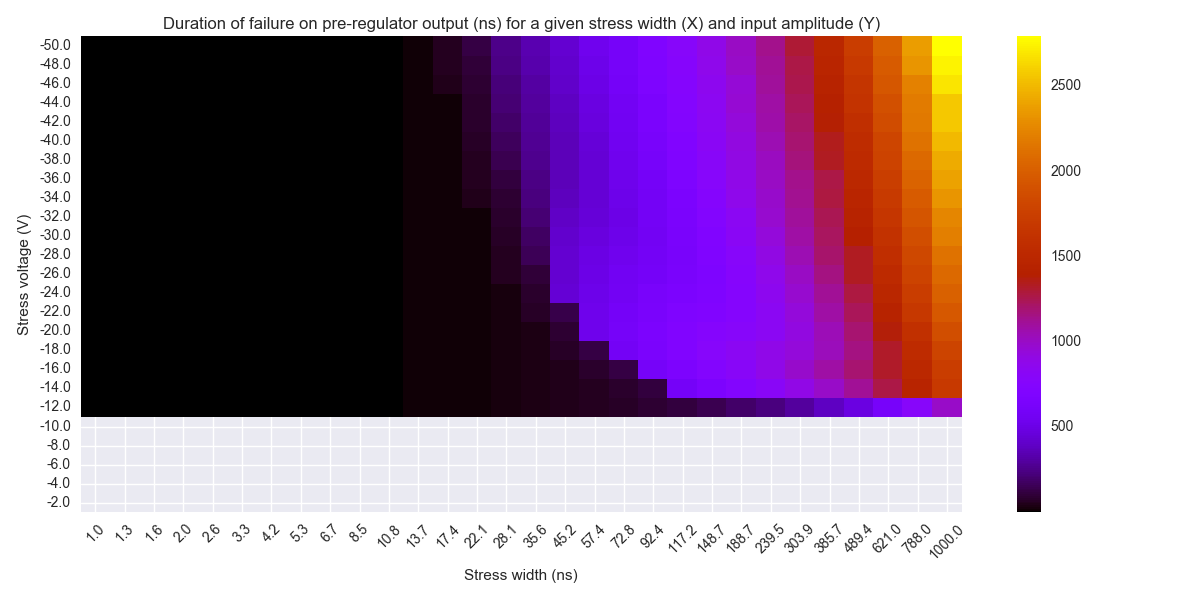
\includegraphics[width=\textwidth]{src/4/figures/preregulator_cz.png}
  \caption{Pre-regulator 9V clamped-output characterization}
  \label{pre_regu_wb}
\end{figure}

\begin{figure}[!h]
  \centering
  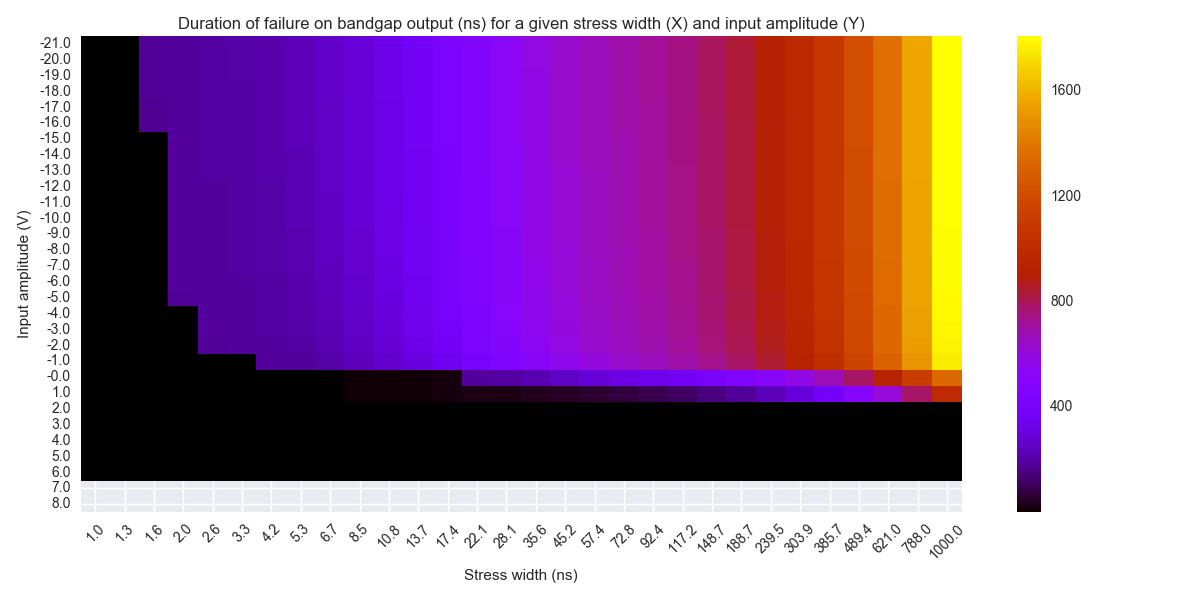
\includegraphics[width=\textwidth]{src/4/figures/bandgap_cz.png}
  \caption{Bandgap 1.0V reference characterization}
  \label{bandgap_wb}
\end{figure}

\begin{figure}[!h]
  \centering
  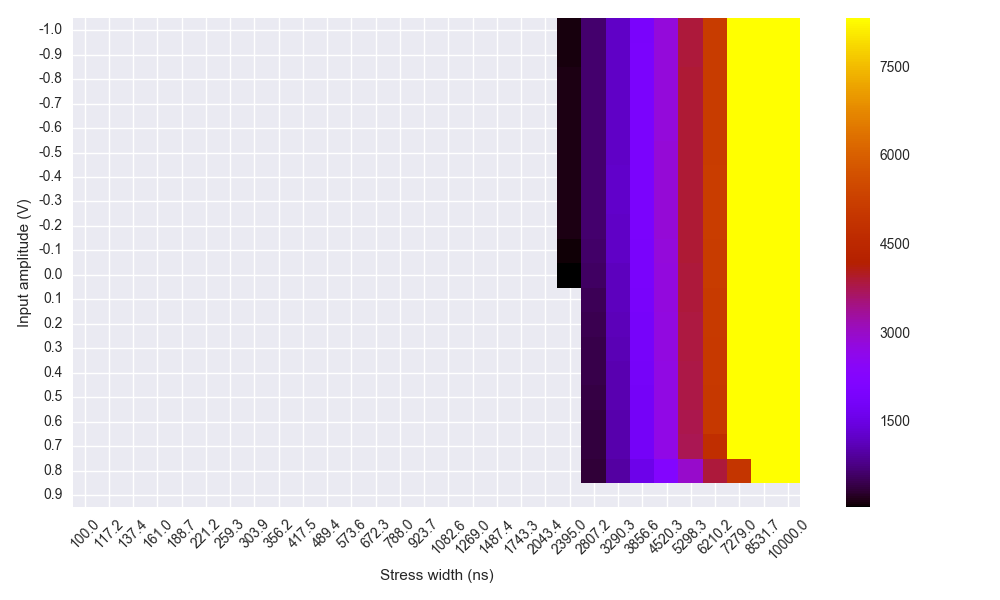
\includegraphics[width=\textwidth]{src/4/figures/regulator_cz.png}
  \caption{Regulator 2.5V supply characterization}
  \label{regu_wb}
\end{figure}

% Characterization done, now perform chaining
After the characterization phase, it is now possible to chain the models together.
The goal is to evaluate the entire function's robustness with the method described in \ref{sec:block-chaining}.
A rectangular pulse is injected on the global input (pre-regulator input).
The chain of models is used to predict, without running any more simulations, the failure or not on the output pin.
For the purpose of this test, the input stress will be generated by a \gls{tlp} generator, producing a pulse of 100ns duration and -30V amplitude.

\begin{figure}[!h]
  \centering
  \includegraphics{src/4/figures/chaining_curves.png}
  \caption{Principle of chaining model curves ?}
  \label{fig:chain-curves}
\end{figure}

% Do it on one pulse config
%TODO: Review values
First, the coordinates (100ns, -30V) are reported on curve \ref{pre_regu_wb}, the first block model of the system.
This point indicates a failure on the output of the pre-regulator, for a duration of 500ns.
The failure criteria is 0V on the output.
This gives the next point coordinates (500 ns, 0V).
This point is reported on the bandgap's model, the next block in the system.
Using these coordinates in the curve \ref{bandgap_wb} indicates a failure on the bandgap output for about 800ns.
Since the failure criteria for the bandgap is 0V on the output, the next point coordinates are (800ns, 0V).
They are used as an input on the final block's model (fig. \ref{regu_wb}).
Reporting those coordinates, no failure is expected on the regulator output.

In conclusion, the model chain estimated that for a -30V 100ns stress on the input, the regulation function will not be at fault (output < 2.1V).

% Same analysis but with a TLP stress that will cause a fail
The same analysis is done for a -30V stress but with a longer width of 1us.
The failure on the pre-regulator is then estimated to last 2300 ns.
In turn, the bandgap is estimated to fail during 3000 ns.
Finally, the output of the regulator and thus the entire function is estimated to fail during 1500ns.

% Perform standard complete simulation for reference
Those results are then tested against a complete simulation of the entire regulation function (all three block).
The simulation circuit is given Fig. \ref{fig:reference_simu_circuit}.
This simulation uses transistor-level block models.
It will serve as a reference to compare the model-chain against it.
%TODO: Speak about simplifications in this circuit. Not consistent with failure case represented in previous chapter

% How will the simulation be conducted
For this simulation, the same input stress are used than previously, and the global output is monitored for failures.
To check the validity of the models at each stage, intermediate voltages are also monitored, at the output of the pre-regulator and the bandgap.
The simulation of the input, pre-regulator output, bandgap output and final (regulator) output are given fig. \ref{fig:reference_simu}.

%TODO: Add perfect sources in schematic
%TODO: Complete schematic with more details
%TODO: Improve figures (text fonts)
\begin{figure}[!h]
  \centering
  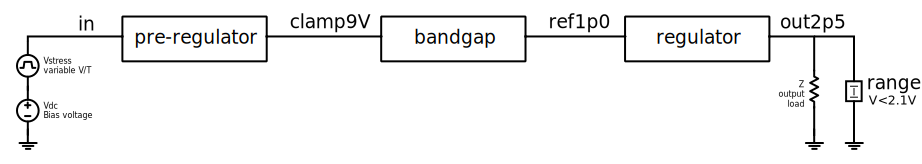
\includegraphics[width=\textwidth]{src/4/figures/complete_simulation_setup.pdf}
  \caption{Complete reference simulation circuit}
  \label{fig:reference_simu_circuit}
\end{figure}

% Result of the simulation
The reference simulation showed that for a -30V 1\textmugreek{}s TLP stress, the output V(out2p5) does not fall below 2.1V.
The minimal value is 2.15V.
As a reminder, with the same conditions, the chain of models estimated the output to go below 2.1V for 1500ns, without informations regarding minimal value.
To understand those differences, intermediate nets are now observed.

% Error at the first block
At the output of the first block (the pre-regulator), the reference simulation shows voltage going below 0V (failure criteria) for 1000ns.
The model predicted 2300 ns.
At the first block's output, there is a factor of 2 between model and reference simulation.

%TODO: To replace with one extracted with perfect sources
%TODO: Fix scale (us instead of ns)
\begin{figure}[!h]
  \centering
  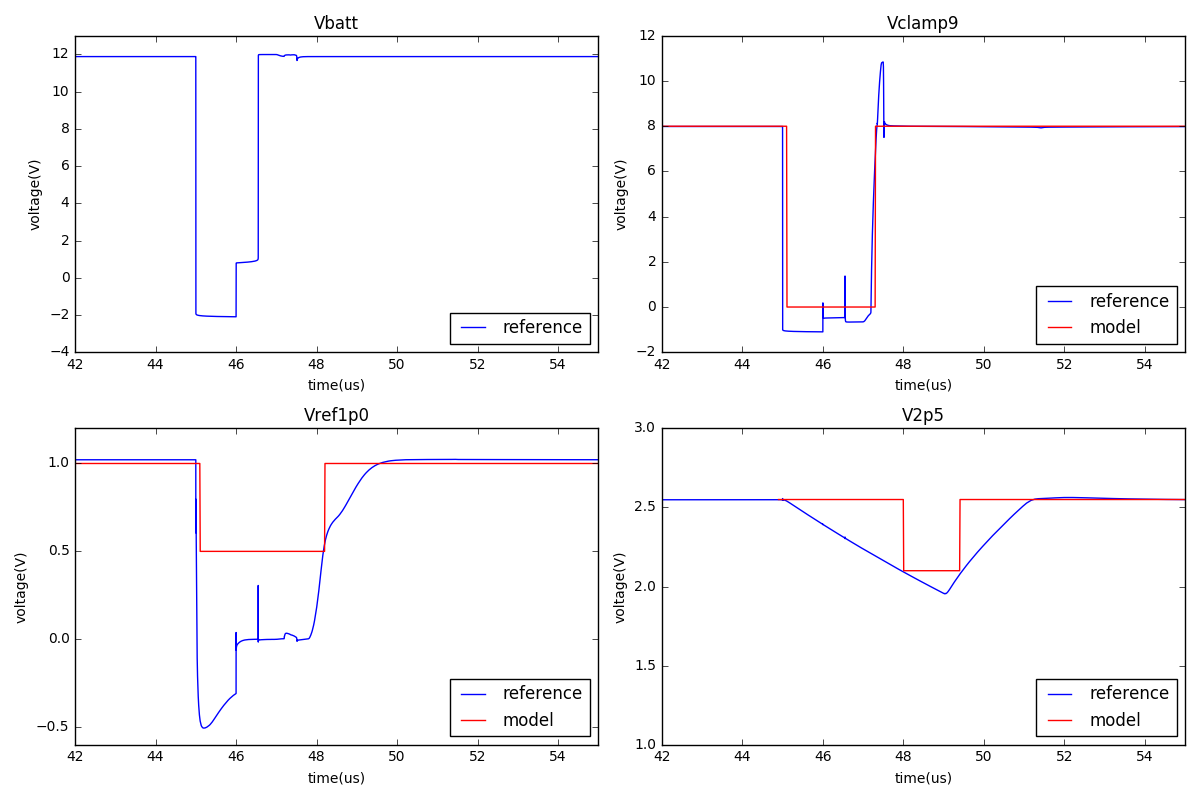
\includegraphics[width=\textwidth]{src/4/figures/total_simulation_30V_1u.png}
  \caption{Reference simulation waveform - TLP stress -30V 1\textmugreek{}s }
  \label{fig:reference_simu}
\end{figure}

% Error at the second block
At the output the second block (bandgap), the reference simulation falls below 0V during approximately 1800 ns.
The minimal reached value is -0.8V
The model predicted the voltage to go below 0V for 3000 ns.
No clear conclusion can be drawn yet on the model validity.

% Test further simulation vs model
To test it further, a set of reference simulations is ran, with variable pulse amplitude and length.
The goal is to get more reference data to test the model against.
For each stress, the result predicted by the model and the reference simulation are compared.

% Preliminary conclusion regarding the results, differences observed
The simulation is ran with stresses ranging from (-2V, 1ns) to (-50V, 1us).
In the case of the reference simulations, no failure is ever recorded.
The models on the opposite predict that in the worst case (-50V, 1us) the regulator's output will go below 2.1V for 2us.

% Observe intermediate nets
Unlike the final output, the full simulation exhibits failures on intermediate nets.
In the worst case (TLP -50V 1us), the first net vlamp9 is disturbed during 1\textmugreek{}s and the second net v1p0 during 2us.
With the model chain, vclamp9 is disturbed during 2800ns and v1p0 for 3200ns.

% Conclusion regarding the results
In conclusion, the model was tested against reference simulations on a wide range of input stresses.
There does not seem to be any clear correlation between the two.
The model seems to not fit the simulation at all, in the current conditions of its extraction.

In regard of these problems, the next section will discuss pitfalls of this bottom-up characterization and modelling method.
Potential workaround will be detailed.
